%%% LaTeX Template: Article/Thesis/etc. with colored headings and special fonts
%%%
%%% Source: http://www.howtotex.com/
%%% Feel free to distribute this template, but please keep to referal to http://www.howtotex.com/ here.
%%% February 2011
%%%
%%% Modified October 2015 by CDM

%%%  Preamble
\documentclass[11pt,letterpaper]{article}
\usepackage[margin=1.0in]{geometry}
\usepackage[T1]{fontenc}
\usepackage[bitstream-charter]{mathdesign}
\usepackage[latin1]{inputenc}
\usepackage{amsmath}
\usepackage{xcolor}
\usepackage{cite}
\usepackage{hyphenat}
\usepackage{graphicx}
\usepackage{float}
\usepackage{subfigure}
\usepackage{sectsty}
\usepackage[compact]{titlesec}
\usepackage[tablegrid]{vhistory}
\allsectionsfont{\color{accentcolor}\scshape\selectfont}

%%% Definitions
\definecolor{accentcolor}{rgb}{0.0,0.0,0.5}
\newcommand{\teamname}{Team Demeter}
\newcommand{\productname}{Polar FarmBot}
\newcommand{\coursename}{CSE 4316: Senior Design I}
\newcommand{\semester}{Fall 2016}
\newcommand{\docname}{System Requirements Specification}
\newcommand{\department}{Department of Computer Science \& Engineering}
\newcommand{\university}{The University of Texas at Arlington}
\newcommand{\authors}{Arun Kalahasti \\ Bipin Ghimire \\ Saman Shrestha \\ Santosh Pradhan \\ Travis Matthews}

%%% Headers and footers
\usepackage{fancyhdr}
	\pagestyle{fancy}						% Enabling the custom headers/footers
\usepackage{lastpage}
	% Header (empty)
	\lhead{}
	\chead{}
	\rhead{}
	% Footer
	\lfoot{\footnotesize \teamname \ - \semester}
	\cfoot{}
	\rfoot{\footnotesize page \thepage\ of \pageref{LastPage}}	% "Page 1 of 2"
	\renewcommand{\headrulewidth}{0.0pt}
	\renewcommand{\footrulewidth}{0.4pt}

%%% Change the abstract environment
\usepackage[runin]{abstract}			% runin option for a run-in title
%\setlength\absleftindent{30pt}			% left margin
%\setlength\absrightindent{30pt}		% right margin
\abslabeldelim{\quad}
\setlength{\abstitleskip}{-10pt}
\renewcommand{\abstractname}{}
\renewcommand{\abstracttextfont}{\color{accentcolor} \small \slshape}	% slanted text

%%% Start of the document
\begin{document}

%%% Cover sheet
{\centering \huge \color{accentcolor} \sc \textbf{\department \\ \university} \par}
\vspace{1 in}
{\centering \huge \color{accentcolor} \sc \textbf{\docname \\ \coursename \\ \semester} \par}
\vspace{0.5 in}
\begin{figure}[h!]
	\centering
   	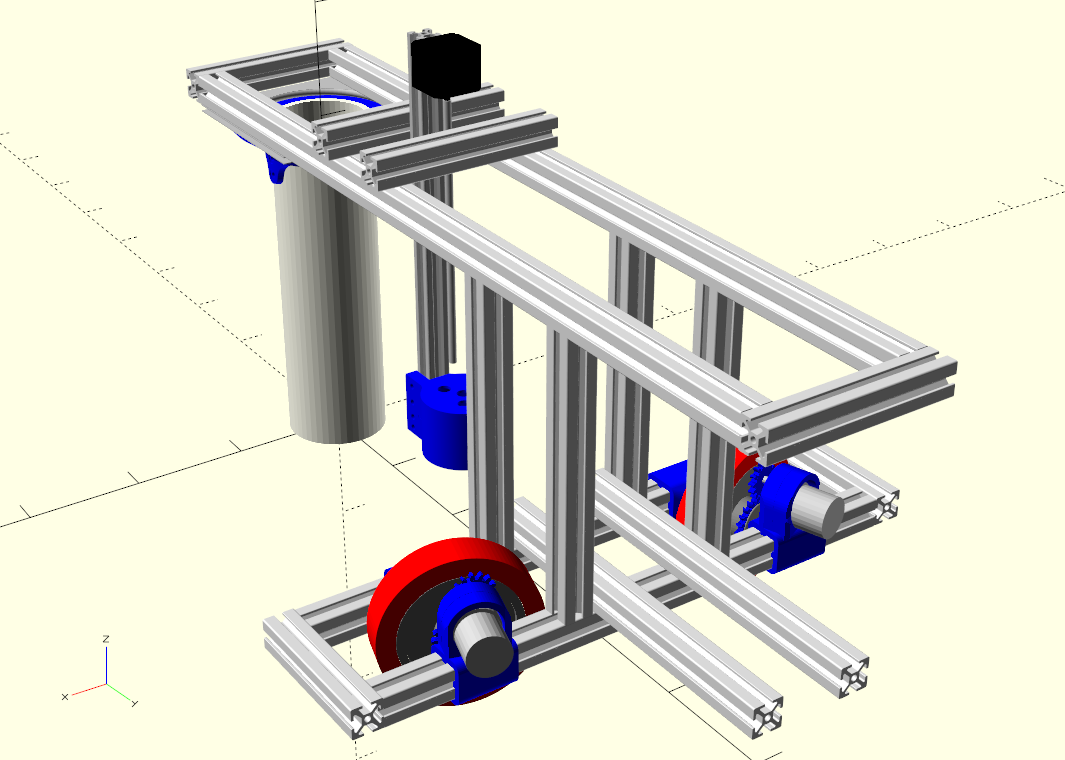
\includegraphics[width=0.60\textwidth]{images/detailed}
\end{figure}
\vspace{0.5 in}
{\centering \huge \color{accentcolor} \sc \textbf{\teamname \\ \productname} \par}
\vspace{0.5 in}
{\centering \large \sc \textbf{\authors} \par}
\newpage


%\vspace{1 in}
%\centerline{January 13th, 2012}
%\newpage

%%% Revision History
\begin{versionhistory}
  	\vhEntry{1.0}{10.25.2016}{TM}{document creation}
\end{versionhistory}
\newpage

%%% Table of contents
\setcounter{tocdepth}{2}
\tableofcontents
\newpage

%%% List of figures and tables (optional)
\listoffigures
%\listoftables
\newpage

\section{Product Concept}
This section will outline the purpose and use of Polar Farmbot and who Polar Farmbot is targeted to. Polar FarmBot is a system that performs basic gardening tasks. Users of the Polar FarmBot will be able to automate the home gardening experience.

\subsection{Purpose and Use}
Polar FarmBot is a CNC robot that automates the agricultural growing process. The robot will plant seeds, water plants, measure soil conditions, and remove weeds. Polar FarmBot will be station in a backyard and will be used to grow various fruits and vegetables such as carrots, lettuce, watermelon, onions, and much more along with all kinds of spices and herbs.

\subsection{Intended Audience}
The target audience for Polar Farmbot would be individuals or small families that are looking to save time in gardening at home. Polar FarmBot is for anyone who loves to garden at home. The robot is intended for general use and anyone can deploy one of these systems and get it up and going in no time.

\newpage
\section{Product Description}
This section provides an overview of Polar FarmBot. It will outline the the primary operational aspects of the product for all users of Polar FarmBot. In addition, there will be key features and functions found in the product, as well as user interfaces are detailed here.

\subsection{Features \& Functions}
Polar FarmBot will be able to plant seeds, water plants, measure soil conditions, and remove weeds. The system will not be able to harvest plants nor remove pests from the plants. Polar FarmBot will have a central pole in which an arm pivots around. The arm will extend outward from the central pole at variable lengths depending on the size specified by the consumer. At the end of the arm there will be a support that extends downward to a set of wheels that allow the arm to move in a circular direction around the central pole. Along the arm there will be a gantry system that will be powered by a motor to move horizontally back and forward on the arm. The gantry will also have a separate motor that will power a separate arm that moves up and down in the vertical direction. Attached to the rod will be the seeder, water pump, and soil monitor tool assembly. Cables and connectors will be routed through the arm, down the central pole, and back out to a control box located just outside the gardening plot.

Within the control box, there will be a motor driver and raspberry pi. The motor driver will power all the motors and sensors on the gantry. The raspberry pi will connect to the internet that will allow for a web based user interface to interact with the system. The control box will also house a power supply that will power all the motors, sensors, motor driver, and raspberry pi. There will also be connectors for the vacuum for picking up seeds and also a connector for water that will allow the robot the ability to water plants. See figure 2A below for a detailed picture of the system

\begin{figure}[h!]
	\centering
   	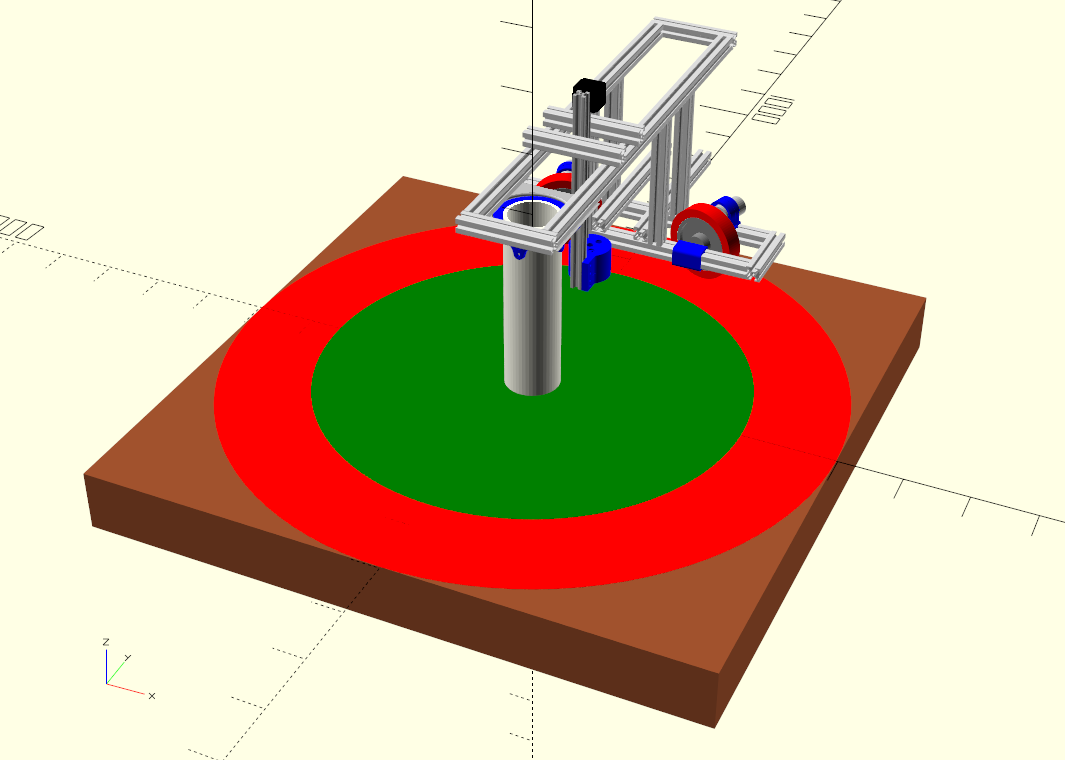
\includegraphics[width=0.60\textwidth]{images/farmbot}
    \caption{Polar FarmBot System Overview}
\end{figure}

\subsection{External Inputs \& Outputs}
Required inputs come directly from the web user interface. A user will outline their plot for their given garden size and farmbot will take care of the rest. The only thing that a user needs to maintain is power to the robot and water. If using the garden hose adapter then maintaining water supply is not necessary. If using the water tank however, then making sure the tank maintains water is on the user.

\subsection{Product Interfaces}
Polar FarmBot will be accessible via the internet. There will be a web service that will be hosted from the Raspberry Pi that will allow for controlling the robot remotely. Along with the web interface, there will also be hard wired buttons for testing the operations of the robot.

\newpage
\section{Customer Requirements}
The Polar FarmBot will be able to plant and monitor the growth of plants without any human supervision. The bot will be able to plant seeds on a 16 feet by 16 feet plot. It will have various functions such as watering the plants, destroying the weeds and many more.

\subsection{Able to plant seeds }
\subsubsection{Description}
The bot will be able to plant the seeds as the customer requires. It will be able to plant any seeds at any of plots within the range of the bot. Polar FarmBot consists of various nozzles, one of which is the seed injector. The seed injector works by using a strong vacuum pump to suction hold onto the tip. The seed injector is 3D printed in the lab and is supposed to be strong and durable. The seed injector will suck in seeds from the seed bin and will plant the seeds on the designated plots.
\subsubsection{Source}
The source of the requirements is the senior design team Demeter.
\subsubsection{Constraints}
The seed injector cannot identify what type of seeds to plant. The user has to put the right seeds in the right seed bin in order to get appropriate results. One might mix variety of seed types into one of the seed bin and have the bot plant whatever it happens to grab but the bot will have no idea of knowing what seed it is planting.
\subsubsection{Standards}
List of applicable standards
\subsubsection{Priority}
The priority of this requirement is critical as the whole idea of the Polar FarmBot depends on the bot being able to grow plants without any human help.

\subsection{Able to water plants}
\subsubsection{Description}
The bot will be able to water the plants once the seeds are sowed. The bot consists of a watering nozzle which will water the plants at certain time of the day. The watering nozzle is 3D printed in the lab. It is connected to the garden hose in the central pole. Once the gantry is connected with the watering nozzle, the bot will start watering the seeds and will water all the seeds that are planted in the plot.
\subsubsection{Source}
The source of the requirements is the senior design team Demeter.
\subsubsection{Constraints}
If any of the plants require more or less water than other plants, the watering nozzle will not be able to detect that. The watering nozzle will water all the plants equally.
\subsubsection{Priority}
The priority of this requirement is critical as if the seeds are not watered well, there is a possibility that the plants might wither off.

\subsection{Check the properties of the soil}
\subsubsection{Description}
The bot will be able to check the properties of the soil for better yield results. The bot consists of a soil sensor tool which is able to accurately read the properties of the soil. The soil sensor tool will give readings like the current amount of moisture on the soil and more. The base for the soil sensor tool is 3D printed in the lab and it will be attached to a soil sensor. The soil sensor works by driving the tool vertically into the soil so that the soil properties can be read accurately.
\subsubsection{Source}
The source of the requirements is the senior design team Demeter.
\subsubsection{Constraints}
The soil sensor tool has to be handled carefully and if the soil sensor cannot be driven directly into the ground, it will give inaccurate readings. One needs to be more careful while handling this equipment as if not handled carefully, the soil sensor circuit board might be damaged.
\subsubsection{Priority}
The priority of this requirement is high, but not critical. Having a soil sensor will help for faster growth of plants and better yields.

\subsection{Kill weeds}
\subsubsection{Description}
The bot will be able to detect and kill weeds as required. Weeds in the plot will be destroyed by either pouring hot water in the weed or will be cut via blades. The blades tool will attach to the gantry and when it operates, it will be able to chop off all the weeds that is detected. The hot water nozzle will be able to kill the weeds by simply pouring hot water in the weeds. The arm will have a raspberry pi camera mounted to it which will detect any weeds that has grown in the plot.
\subsubsection{Source}
The source of the requirements is the senior design team Demeter.
\subsubsection{Constraints}
The blade tool has to be constantly maintained and checked for rust. If the weeds are too strong then the blade might not be able to chop off the weed as desired. While pouring the hot water into the weeds, we need to make sure that none of the hot water affects the plants and if miscalculated, the bot might hot water the plants instead of the weeds and kill the plants.
\subsubsection{Priority}
The priority of this requirement is high. If weeds are let to grow and not managed in time, it will deplete the quality of the soil and the field will look unmanaged.

\subsection{Create Web application}
\subsubsection{Description}
The FarmBot will be controlled via web application. The web app allows you to easily configure and control your FarmBot from a web browser on your laptop, tablet, or smartphone. The application features real-time manual controls and logging, a sequence builder for creating custom routines for FarmBot to execute, and manage your farm. FarmBot's Raspberry Pi is used to maintain a connection and synchronize with the web application. Arduino firmware will be used for physically operating FarmBot's hardware, tools, sensors, and other electronics. It receives G and F codes from FarmBot Raspberry Pi Controller via the USB serial connection, and then moves the motors and reads and writes pins accordingly. It also sends collected data from the rotary encoders and pin reads back to the Raspberry Pi.
\subsubsection{Source}
The source of the requirements is the senior design team Demeter.
\subsubsection{Constraints}
The software needs to be maintained constantly and any problem in the software will halt all the functions of the hardware.
\subsubsection{Priority}
The priority of this requirement is critical. The software is one of the most important aspect of the whole project and failing to make a functioning software will cause the whole project to fail.

\newpage
\section{Packaging Requirements}
The hardware components of the Polar FarmBot at first will be disassembled and all components will be packed in boxes. All components will be bubble wrapped to control any damage done during shipping and handling. All the complex components will already be assembled and the customers will only need to assemble the arms to the central pole and attach the gantry to the arm. Detailed instructions would be provided inside the box on how to attach each piece to other. The software will be a web based application. A CD will be provided to the customer with the software with easy installation guide.

\subsection{Hardware Packaging}
\subsubsection{Description}
All the hardware components will packed separately. There will be an instruction manual to assemble all the parts. The arms will attach to the central pole with a few bolts and nuts. The end piece will already be assembled and all the user has to do is to attach ii to the arms. The gantry will be assembled as well and all that is need to be done is attach to the arm. All the components like the seed injector, the weed killer will be already assembled and ready for use. All the 3D printed components will be available for use as well. All the components will be bubble wrapped and boxed properly to protect from external damage while shipping and handling. Enough nuts and bolts would be provided for complete assembly.
\subsubsection{Source}
The source of this requirement is the Senior Design Team Demeter.
\subsubsection{Constraints}
Even though the assembly of the components is supposed to be simple and easy some people might find it confusing. And even with all the packaging, some parts might get damaged during shipping and handling.
\subsubsection{Priority}
The priority for the packaging will be critical. It is very important that the software operates fully for the hardware to start working in its full capacity.

\subsection{Software Distribution}
\subsubsection{Description}
The required software will be installed in a CD and provided to the user. There will be an easy installation process. Once the CD is loaded in a computer the user has to follow few simple guides and the software will be ready to use.
\subsubsection{Source}
The source of this requirement is the Senior Design Team Demeter.
\subsubsection{Constraints}
The software would require Windows 7 and up or MAC with macOS 10 or higher.
\subsubsection{Priority}
The priority for the packaging will be critical. It is very important that the software operates fully for the hardware to start working in its full capacity.

\newpage
\section{Performance Requirements}
\subsection{Rotation Speed}
\subsubsection{Description}
The Farmbot must be able to move at least 12 feet per minute on the outer edge. 
\subsubsection{Source}
Defined by Team Demeter
\subsubsection{Constraints}
Motor rotation speed will limit the total speed.
\subsubsection{Priority}
Low priority

\subsection{Time to plant the complete plot}
\subsubsection{Description}
The Polar FarmBot will be able to plant the entire plot within 1 hour. Similarly the bot will finish watering plants in 90 minutes.
\subsubsection{Source}
Defined by Team Demeter
\subsubsection{Constraints}
Motor rotation speed will limit the total speed. Time might vary depending on the condition of the soil, temperature and other factors.
\subsubsection{Priority}
Medium priority

\subsection{Power Management}
\subsubsection{Description}
The Polar FarmBot will need a constant supply of power in order to function properly.
\subsubsection{Source}
Defined by Team Demeter
\subsubsection{Constraints}
Power will need to be supplied from a grid or a solar panel.
\subsubsection{Priority}
Medium priority

\newpage
\section{Safety Requirements}
Polar FarmBot is being designed in a way that will have least safety issue.

\subsection{Description}
The bot will not have any sharp edges.
All electric currents are housed in waterproof enclosures
Speed of arm will be slow enough that being hit by the bots arm will not cause physical damage
\subsubsection{Source}
The source of the requirements are the senior design team Demeter.
\subsubsection{Constraints}
\subsubsection{Standards}
\subsubsection{Priority}
Priority will be to make sure the Polar FarmBot will not have any serious safety issue.

\newpage
\section{Maintenance \& Support Requirements}
The Demeter Team believes that the polar FarmBot will be able to help the customers to produce food both on the small and large scale. We have set up a milestone that will be achieved on the success of this project. The milestone is to come up with a minimum workable product like FarmBot Genesis. This will help prove or disprove the workability of this technology.
This section of System Requirement Specification includes the list and description of Maintenance and Support Requirements for the project. This section provides all the required information about how to build up the whole product and implement all the required maintenance after the delivery of the product. This section includes list of requirements such as documentation of the source code which is well commented and easy to go over; required support/troubleshooting manuals/guides that describes how to use the delivered product and how to troubleshoot for the small problems encountered during its use; specific/unique tools required for maintenance; and specific software/environment required for maintenance.

\subsection{SOURCE CODE}
\subsubsection{Description}
Source code will be made available to the user on the final delivery. Source code will be well commented so that it is easily readable by the user. Each functionality will be made logically and technically simple using appropriate format of comments.
\subsubsection{Source}
The source of the requirements is the senior design team Demeter.
\subsubsection{Constraints}
None
\subsubsection{Priority}
High

\subsection{USER MANUAL}
\subsubsection{Description}
Product will be delivered with a simple and easy to follow user manual. It will provide guidelines on how to use the product. It will also include various sections like table of content, system overview, getting started and glossary. Also, explicit instructions to use each major component will be in separate section. 
\subsubsection{Source}
The source of the requirements is the senior design team Demeter.
\subsubsection{Constraints}
User manual will be available only in English language.
\subsubsection{Standards}
Standard American English
\subsubsection{Priority}
Moderate

\subsection{TROUBLESHOOTING GUIDE}
\subsubsection{Description}
Troubleshooting Guide will be made available to the customer on the final delivery of the product. It will be simple and easy to follow guidelines that will help user on problem detection. Unlike User Manual, it will help user to carry troubleshooting on the minor problems with its well formatted and diagrammatic guidelines thus, removing the potential harms.
\subsubsection{Source}
The source of the requirements is the senior design team Demeter.
\subsubsection{Constraints}
Like User Manual, Troubleshooting Guide will be available only in English Language.
\subsubsection{Standards}
Standard American English
\subsubsection{Priority}
High

\subsection{DOCUMENTATION AVAILABILITY}
\subsubsection{Description}
Documentation done throughout the development phase of this project will be included on the final delivery of this product. It will provide customers ideas on how the whole system is built from the scratch. It will include Project Charter, System Requirements Specification, Architectural Design Specifications, Detailed Design Specifications, and System Test Plan. It will be well formatted and easy to understand.
\subsubsection{Source}
The source of the requirements is the senior design team Demeter.
\subsubsection{Constraints}
None
\subsubsection{Standards}
Standard American English
\subsubsection{Priority}
Moderate

\subsection{DATABASE MAINTENANCE}
\subsubsection{Description}
Data related to the product will be stored using MYSQL database. Demeter Team will be responsible for creation and maintenance of the database throughout the product development phase. But customers will be responsible for the maintenance of the database after the delivery of the product.
\subsubsection{Source}
Customers
\subsubsection{Constraints}
None
\subsubsection{Priority}
High

\subsection{HARDWARE SUPPORT AND MAINTENANCE GUIDE}
\subsubsection{Description}
Hardware Support and Maintenance Guide will be provided to the customers at the end of the final delivery of the product. It will contain the tips and techniques to keep the FarmBot running smooth for years to come and to keep it operating like the day it was installed. Some of the tips and techniques will include ways to keep FarmBot clean, to tighten loose screws, to inspect for damage and to remove magnetic debris buildup in the tools.
\subsubsection{Source}
Customer
\subsubsection{Constraints}
Maintenance Guide will be available only in English language.
\subsubsection{Priority}
High

\subsection{DEMONSTRATION AND TRAINING}
\subsubsection{Description}
Demonstration and Training will be offered to the customer showing how the FarmBot operates overall. They can also refer to the User Manual for further help.
\subsubsection{Source}
The source of the requirements is the senior design team Demeter.
\subsubsection{Constraints}
None
\subsubsection{Priority}
Moderate
\newpage
\section{Other Requirements}
\subsection{LARGE SCALE FARMBOT (EXTENSION)}
\subsubsection{Description}
The FarmBot will be extendable to at least cover a 16 feet by 16 feet plot and will able be used in large scale to minimize the manpower as per the customer needs. The same working principles will be applied in the large scale FarmBot too. This feature will not be included in the current version.
\subsubsection{Source}
Customer
\subsubsection{Constraints}
The production cost will be higher.
\subsubsection{Priority}
Moderate

\subsection{Assembly Instructions}
\subsubsection{Description}
Assembly instructions must contain enough detail for a technically literate user to construct the physical robot as well as install any required softwares.
\subsubsection{Source}
Assembly instructions will be provided by Team Demeter
\subsubsection{Constraints}
Assembly instructions must be clear enough to follow. Instructions may be transmitted through static mediums.
\subsubsection{Priority}
Assembly instructions are high priority, but not critical for completion of the project.

\subsection{Assembly Instructions - Parts List}
\subsubsection{Description}
The hardware assembly must contain a complete and comprehensive list of all parts and a minimum count needed for complete construction of the robot.
\subsubsection{Source}
Parts list will be provided by Team Demeter
\subsubsection{Constraints}
The parts list must contain enough detail to order specific parts to ensure the customer will order the correct parts if they wish to source their own components.
\subsubsection{Priority}
A parts list is critical for replication of the project. Builders will not know what components and how many may be required without a parts list.

\subsection{Assembly Instructions - Software Configuration}
\subsubsection{Description}
The assembly instructions should contain references to the locations, details, and purposes of configuration as they differ from default settings. The assembly instructions will not contain directions on installing or uploading software to the hardware platforms.
\subsubsection{Source}
A software configuration will be provided by Team Demeter
\subsubsection{Constraints}
An unclear guide can lead to improper configuration and hardware damage.
\subsubsection{Priority}
A software configuration guide is not critical for deployment.

\newpage
\section{Future Items}

\subsection{Portable/Reusable Body}
\subsubsection{Description}
The main body of the Polar FarmBot should be movable from one plot to another. The mobile body of the Polar FarmBot must be self contained and require nothing from the support post but a supply of electricity and liquids to dispense. Once the FarmBot has been given a layout for a new plot, it should be able to operate on the contents of that plot without reconfiguration beyond plot selection when moved back to that plot.
\subsubsection{Source}
Plans for a Portable Polar FarmBot will be provided by Team Demeter
\subsubsection{Constraints}
In order to be mobile the Polar FarmBot must be able to disconnect from any permanently installed fixtures. All connectors for liquid and electrical input must have the ability to connect and disconnect. Optionally, the procedure can be designed to be done without tools.
\subsubsection{Priority}
The mobility of the FarmBot is low priority and not necessary to the core functionality of the machine.

\newpage

%%% References
\bibliographystyle{plain}
\bibliographystyle{reference/IEEEtran_custom}
\bibliography{reference/refs}{}

\end{document}
